\section*{A really good Separation system}

The separation of p-nitrotoluene from a liquid mixture of predominantly p-nitrotoluene and m-nitrotoluene with trace amounts of o-nitrotoluene has been selected for detailed design. The choice has been because p-nitrotoluene is an essential precursor for production of both aminobenzaldehyde and aminobenzoic acid and needs to be at least 90\% purity. Due to the negligible difference in boiling points yet sizeable difference in melting points of p-nitrotoluene and m-nitrotoluene, crystallisation has been chosen as the separation methodology. A cooling melt crystalliser has been designed to be implemented downstream of distillation column S103, where solid p-nitrotoluene would crystallise out from the liquid mixture. A subsequent hydraulic wash column has been designed immediately downstream of the crystalliser to recover pure solid p-nitrotoluene from the slurry. 


The liquid mixture to be separated has been modelled as (p-nitrotoluene and m-nitrotoluene) binary system because the presence of o-nitrotoluene is negligible. This mixture exhibits a eutectic-forming solid-liquid phase behaviour, where p-nitrotoluene is able to crystallise from the mixture liquid as pure solid. The crystalliser has been modelled as operating under mixed suspension mixed product removal (MSMPR) mode, where perfect mixing is assumed and the crystalliser operates at outlet conditions. Kinetics for crystal nucleation and growth were obtained from the literature and used for . An agitator has been implemented to achieve MSMPR operation and uniform temperature, and its geometry aims at minimising fouling in the vessel. To provide cooling for the crystalliser, a half pipe cooling coil surrounds the vessel through which cooling medium of 10\% ethylene glycol aqueous solution flows at \SI{7}{L/s} with temperature of \SI{274}{K}. Figure \ref{fig:crystalliser schematic executive} provides a 3D overview of the crystalliser design.


The hydraulic wash column has been modelled based on a volume and a force balance. Hydraulic wash columns used for ultrapurification have been proven to achieve 99.9\% separation of solid organics from liquid in continuous operations. For the design, an overall 99.9 \% p-nitrotoluene recovery in the final product outlet has been assumed. The diameter and steer flow rate were varied across the length of the column to observe the effect on the pressure drop . The pressure drop at various locations of the column were observed as key variables (the diameter and steer flow rate) were varied. From this a suitable diameter of 0.17 m and steer flow rate  of $2.65 \times 10^{-5} m^{3}/s$ was chosen. Finally, a sensitivity analysis was conducted on the Kozeny constant to see how this impacts the pressure drop across the column.


\begin{figure}[h]
    \centering
    \includesvg[scale=0.3,inkscapelatex=false]{chapters/3-separation/figures/Crystalliser_schematic.svg}
    \caption{Schematics for the designed crystalliser vessel: (i) perspective view; (ii) section view.}
    \label{fig:crystalliser schematic executive}
\end{figure}

\begin{figure}[h]
    \centering
    \includesvg[scale=0.3,inkscapelatex=false]{chapters/3-separation/figures/Wash_column_schematic_executive.svg}
    \caption{Schematics for the hydraulic wash column: (i) perspective (ii) right-side section (iii) front section.}
    \label{fig:wash column schematic executive}
\end{figure}

\begin{figure*}[t!]
    \centering
    \begin{subfigure}[t]{0.5\textwidth}
        \centering
        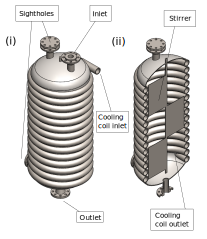
\includegraphics[width=\linewidth]{chapters/3-separation/figures/Crystalliser_schematic.svg}
        \caption{$CO_2$ plume model}
    \end{subfigure}%
    ~ 
    \begin{subfigure}[t]{0.5\textwidth}
        \centering
        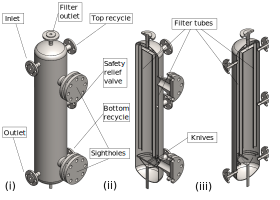
\includegraphics[width=\linewidth]{chapters/3-separation/figures/Wash_column_schematic_executive.svg}
        \caption{$NO_2$ plume model}
    \end{subfigure}
\end{figure*}